\documentclass[11pt, oneside]{article}   	% use "amsart" instead of "article" for AMSLaTeX format
\usepackage{geometry}                		% See geometry.pdf to learn the layout options. There are lots.
\geometry{letterpaper}                   		% ... or a4paper or a5paper or ... 
%\geometry{landscape}                		% Activate for for rotated page geometry
%\usepackage[parfill]{parskip}    		% Activate to begin paragraphs with an empty line rather than an indent
\usepackage{graphicx}				% Use pdf, png, jpg, or eps§ with pdflatex; use eps in DVI mode
								% TeX will automatically convert eps --> pdf in pdflatex		
\usepackage{amssymb}
\usepackage{amsmath}

\title{Ellipse equations}
%\author{The Author}
\date{}							% Activate to display a given date or no date

\graphicspath{{/Users/telliott_admin/Dropbox/Tex/png/}}
\begin{document}

\maketitle
%\section{}
% \subsection*{R code}
% \begin{lstlisting}  \end{lstlisting}
% \begin{center} 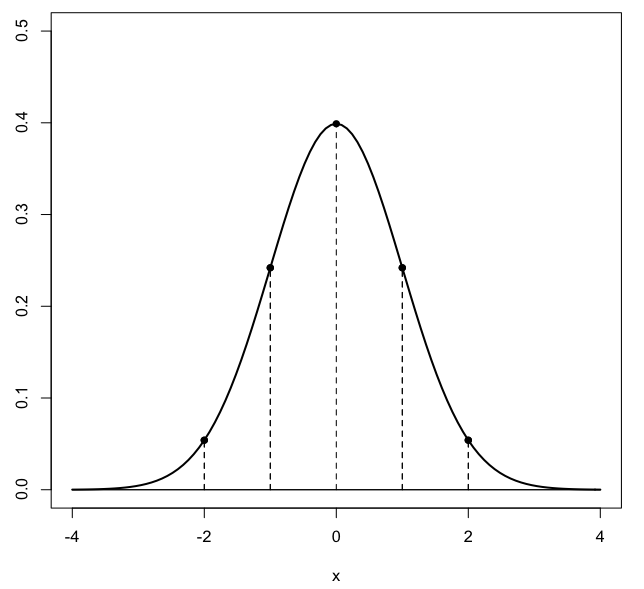
\includegraphics [scale=0.4] {gauss3.png} \end{center}
% \begin{bmatrix} a  &  b \\ c  &  d \end{bmatrix}
% \bigg |_

\large
\noindent
The standard equation for a simple ellipse (aligned with the x- and y-axes) is 
\[ \frac{x^2}{a^2} + \frac{y^2}{b^2} = 1 \]
From the formula it is easy to see that when
\[ x=0; \ \  y = \pm b \]
and similarly when 
\[ y=0; \ \   x = \pm a\]

\begin{center} 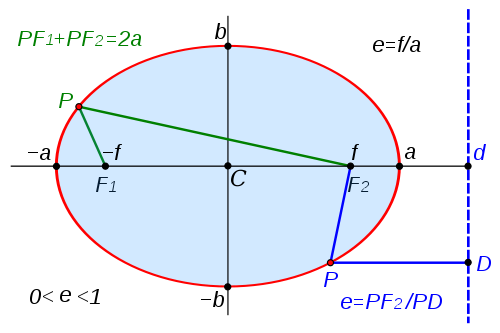
\includegraphics [scale=0.5] {ellipse2.png} \end{center}
The graphic, which is from wikipedia, shows a typical ellipse.  The geometric definition of an ellipse is the set of points which has
\[ PF_1 + PF_2 = const \]
The sum of the distances from any point to each of the two foci is a constant.  The foci lie on the semi-major axis (the long axis of the ellipse), which here is the x-axis.  The formula for the focal distance is
\[ c = \sqrt{a^2 - b^2} \]
For example, if $a=5$ and $b=3$ then $c=4$, so the foci are the two points $(0,-c), (0,c)$.  (Some folks switch the labels $a$ and $b$ depending on the orientation of this axis, but I find it confusing).

The distance from $F_1$ to $P$ ($P_x > 0$) is 
\[ \sqrt{(x + c)^2 + y^2} \]

and from $F_2$ it is
\[  \sqrt{(x - c)^2 + y^2} \]

This sum is a constant, and equal to $2a$ as seen from the point $P=(a,0)$
\[ PF_1 + PF_2 = a - c + a + c = 2a \]

The relation to $b$ can be seen from the point $Q=(0,b)$ where 
\[ PF_1 + PF_2 = 2\sqrt{b^2 + c^2} = 2a \]
\[ b^2 + c^2 = a^2 \]
Given $a$ and $b$ one can then find $c$ easily.

\subsection*{Additional comments}
The first comment is that just as for the other quadratic formulas, one can move the center of the ellipse by including offsets
\[ \frac{(x-h)^2}{a^2} + \frac{(y-k)^2}{b^2} = 1 \]
When presented with an equation in which terms like $-2xh$ or $-2yk$ present, you need to "complete the square" to rearrange the terms as $(x-h)^2$ and $(y-k)^2$, respectively.

Recall that if
\[ Ax^2 + Bxy + Cy^2 + Dx + Ey + F =0 \]
the "discriminant" is $B^2 - 4AC$ and if this is $<0$, then the equation is an ellipse.  The presence of an $xy$ term indicates a rotated quadratic (though not necessarily an ellipse).

\subsection*{Parametric equations}
These are simply
\[ x = a \ cos\theta \]
\[ y = b \ sin\theta \]
It can be verified easily that these solve the basic equation
\[ \frac{x^2}{a^2} + \frac{y^2}{b^2} = 1 \]
and note, for example that if $\theta=\pi/4$ then $x = a/\sqrt{2}; \ \ y = b/\sqrt{2}$.


\subsection*{Derivation of the equation of the ellipse}

Now we just do some algebra.  Rearrange
\[ \sqrt{(x - c)^2 + y^2} = 2a - \sqrt{(x + c)^2 + y^2} \]
Square both sides
\[ (x - c)^2 + y^2 = 4a^2 - 4a \sqrt{(x + c)^2 + y^2} + (x+c)^2 + y^2 \]
Expand $(x \pm c)^2$:
\[ x^2 - 2xc + c^2 + y^2 = 4a^2 - 4a \sqrt{(x + c)^2 + y^2} + x^2 + 2xc + c^2 + y^2 \]
Cancel $x^2$, $y^2$ and $c^2$ and move $2xc$ to the left-hand side
\[ -4xc = 4a^2 - 4a \sqrt{(x + c)^2 + y^2} \]
\[ a^2 + xc = a \sqrt{(x + c)^2 + y^2} \]
Square again
\[ a^4 + 2a^2xc + x^2c^2 = a^2(x^2 + 2xc + c^2 + y^2) \]
\[ a^4 + 2a^2xc + x^2c^2 = a^2x^2 + 2a^2xc + a^2c^2 + a^2y^2 \]
Cancel $2a^2xc$
\[ a^4 + x^2c^2 = a^2x^2 + a^2c^2 + a^2y^2 \]
Gather $x^2$ terms on the left-hand side
\[ a^2x^2 - x^2c^2 = a^4 - a^2c^2 - a^2y^2 \]
\[ (a^2 - c^2)x^2 = (a^2 - c^2)a^2 - a^2y^2  \]
Recall that $c^2 = a^2 - b^2$ so $b^2 = a^2 - c^2$
\[ b^2x^2 = b^2a^2 - a^2y^2  \]
\[ \frac{b^2x^2}{a^2} = b^2 - y^2  \]
\[ \frac{x^2}{a^2} + \frac{y^2}{b^2} = 1  \]



\end{document}  